% Options for packages loaded elsewhere
\PassOptionsToPackage{unicode}{hyperref}
\PassOptionsToPackage{hyphens}{url}
%
\documentclass[
  14pt,
  letterpaper,
  ignorenonframetext,
  aspectratio=169,
]{beamer}
\usepackage{pgfpages}
\setbeamertemplate{caption}[numbered]
\setbeamertemplate{caption label separator}{: }
\setbeamercolor{caption name}{fg=normal text.fg}
\beamertemplatenavigationsymbolsempty
% Prevent slide breaks in the middle of a paragraph
\widowpenalties 1 10000
\raggedbottom
\setbeamertemplate{part page}{
  \centering
  \begin{beamercolorbox}[sep=16pt,center]{part title}
    \usebeamerfont{part title}\insertpart\par
  \end{beamercolorbox}
}
\setbeamertemplate{section page}{
  \centering
  \begin{beamercolorbox}[sep=12pt,center]{part title}
    \usebeamerfont{section title}\insertsection\par
  \end{beamercolorbox}
}
\setbeamertemplate{subsection page}{
  \centering
  \begin{beamercolorbox}[sep=8pt,center]{part title}
    \usebeamerfont{subsection title}\insertsubsection\par
  \end{beamercolorbox}
}
\AtBeginPart{
  \frame{\partpage}
}
\AtBeginSection{
  \ifbibliography
  \else
    \frame{\sectionpage}
  \fi
}
\AtBeginSubsection{
  \frame{\subsectionpage}
}

\usepackage{amsmath,amssymb}
\usepackage{lmodern}
\usepackage{iftex}
\ifPDFTeX
  \usepackage[T1]{fontenc}
  \usepackage[utf8]{inputenc}
  \usepackage{textcomp} % provide euro and other symbols
\else % if luatex or xetex
  \usepackage{unicode-math}
  \defaultfontfeatures{Scale=MatchLowercase}
  \defaultfontfeatures[\rmfamily]{Ligatures=TeX,Scale=1}
  \setmainfont[BoldFont = SF Pro Text Semibold, Scale =
MatchLowercase]{SF Pro Text Light}
\fi
\usecolortheme{wolverine}
\usefonttheme{serif} % use mainfont rather than sansfont for slide text
\useinnertheme{default}
% Use upquote if available, for straight quotes in verbatim environments
\IfFileExists{upquote.sty}{\usepackage{upquote}}{}
\IfFileExists{microtype.sty}{% use microtype if available
  \usepackage[]{microtype}
  \UseMicrotypeSet[protrusion]{basicmath} % disable protrusion for tt fonts
}{}
\makeatletter
\@ifundefined{KOMAClassName}{% if non-KOMA class
  \IfFileExists{parskip.sty}{%
    \usepackage{parskip}
  }{% else
    \setlength{\parindent}{0pt}
    \setlength{\parskip}{6pt plus 2pt minus 1pt}}
}{% if KOMA class
  \KOMAoptions{parskip=half}}
\makeatother
\usepackage{xcolor}
\newif\ifbibliography
\setlength{\emergencystretch}{3em} % prevent overfull lines
\setcounter{secnumdepth}{-\maxdimen} % remove section numbering


\providecommand{\tightlist}{%
  \setlength{\itemsep}{0pt}\setlength{\parskip}{0pt}}\usepackage{longtable,booktabs,array}
\usepackage{calc} % for calculating minipage widths
\usepackage{caption}
% Make caption package work with longtable
\makeatletter
\def\fnum@table{\tablename~\thetable}
\makeatother
\usepackage{graphicx}
\makeatletter
\def\maxwidth{\ifdim\Gin@nat@width>\linewidth\linewidth\else\Gin@nat@width\fi}
\def\maxheight{\ifdim\Gin@nat@height>\textheight\textheight\else\Gin@nat@height\fi}
\makeatother
% Scale images if necessary, so that they will not overflow the page
% margins by default, and it is still possible to overwrite the defaults
% using explicit options in \includegraphics[width, height, ...]{}
\setkeys{Gin}{width=\maxwidth,height=\maxheight,keepaspectratio}
% Set default figure placement to htbp
\makeatletter
\def\fps@figure{htbp}
\makeatother

\let\Tiny=\tiny

\usepackage{MnSymbol}
\usepackage{amssymb}% http://ctan.org/pkg/amssymb
\usepackage{pifont}% http://ctan.org/pkg/pifont
\newcommand{\cmark}{\ding{51}}%
\newcommand{\xmark}{\ding{55}}%

\DeclareSymbolFont{symbolsC}{U}{txsyc}{m}{n}
\DeclareMathSymbol{\boxright}{\mathrel}{symbolsC}{128}
\DeclareMathAlphabet{\mathpzc}{OT1}{pzc}{m}{it}

\setlength{\parskip}{1.5ex plus 0.5ex minus 0.2ex}
\linespread{1.1}

\AtBeginSection[]
{
\begin{frame}
	\Huge{\color{darkblue} \insertsection}
\end{frame}
}

\renewenvironment*{quote}	
	{\list{}{\rightmargin   \leftmargin} \item } 	
	{\endlist }

\definecolor{darkgreen}{rgb}{0,0.7,0}
\definecolor{darkblue}{rgb}{0,0,0.8}

\usepackage[italic]{mathastext}
\usepackage{nicefrac}
\usepackage{istgame}

\setbeamertemplate{caption}{\raggedright\insertcaption} 
\setbeamertemplate{itemize item}[circle]
\setbeamertemplate{footline}[frame number]{}

\mode<handout>{\pgfpagesuselayout{6 on 1}[letterpaper, border shrink=8mm]}
  \AtBeginSection{
          \begin{frame}
              \tableofcontents[currentsection]
          \end{frame}
       }

\usepackage{etoolbox}
\AfterEndEnvironment{description}{\vspace{9pt}}
\AfterEndEnvironment{oltableau}{\vspace{9pt}}
\BeforeBeginEnvironment{oltableau}{\vspace{9pt}}
\AfterEndEnvironment{center}{\vspace{9pt}}
\BeforeBeginEnvironment{tabular}{\vspace{9pt}}
\AfterEndEnvironment{longtable}{\vspace{-6pt}}

\useoutertheme[subsection = false]{miniframes}

\let\olditem\item
\renewcommand{\item}{%
\olditem\vspace{6pt}}
\usepackage{booktabs}
\usepackage{longtable}
\usepackage{array}
\usepackage{multirow}
\usepackage{wrapfig}
\usepackage{float}
\usepackage{colortbl}
\usepackage{pdflscape}
\usepackage{tabu}
\usepackage{threeparttable} 
\usepackage{threeparttablex} 
\usepackage[normalem]{ulem} 
\usepackage{makecell}
\usepackage{xcolor}
\usepackage{ulem}

\setlength\heavyrulewidth{0ex}
\setlength\lightrulewidth{0.08ex}

\aboverulesep=0ex
\belowrulesep=0ex
\renewcommand{\arraystretch}{1.2}
\usepackage{booktabs}
\usepackage{longtable}
\usepackage{array}
\usepackage{multirow}
\usepackage{wrapfig}
\usepackage{float}
\usepackage{colortbl}
\usepackage{pdflscape}
\usepackage{tabu}
\usepackage{threeparttable}
\usepackage{threeparttablex}
\usepackage[normalem]{ulem}
\usepackage{makecell}
\usepackage{xcolor}
\makeatletter
\makeatother
\makeatletter
\makeatother
\makeatletter
\@ifpackageloaded{caption}{}{\usepackage{caption}}
\AtBeginDocument{%
\ifdefined\contentsname
  \renewcommand*\contentsname{Table of contents}
\else
  \newcommand\contentsname{Table of contents}
\fi
\ifdefined\listfigurename
  \renewcommand*\listfigurename{List of Figures}
\else
  \newcommand\listfigurename{List of Figures}
\fi
\ifdefined\listtablename
  \renewcommand*\listtablename{List of Tables}
\else
  \newcommand\listtablename{List of Tables}
\fi
\ifdefined\figurename
  \renewcommand*\figurename{Figure}
\else
  \newcommand\figurename{Figure}
\fi
\ifdefined\tablename
  \renewcommand*\tablename{Table}
\else
  \newcommand\tablename{Table}
\fi
}
\@ifpackageloaded{float}{}{\usepackage{float}}
\floatstyle{ruled}
\@ifundefined{c@chapter}{\newfloat{codelisting}{h}{lop}}{\newfloat{codelisting}{h}{lop}[chapter]}
\floatname{codelisting}{Listing}
\newcommand*\listoflistings{\listof{codelisting}{List of Listings}}
\makeatother
\makeatletter
\@ifpackageloaded{caption}{}{\usepackage{caption}}
\@ifpackageloaded{subcaption}{}{\usepackage{subcaption}}
\makeatother
\makeatletter
\@ifpackageloaded{tcolorbox}{}{\usepackage[many]{tcolorbox}}
\makeatother
\makeatletter
\@ifundefined{shadecolor}{\definecolor{shadecolor}{rgb}{.97, .97, .97}}
\makeatother
\makeatletter
\makeatother
\ifLuaTeX
  \usepackage{selnolig}  % disable illegal ligatures
\fi
\IfFileExists{bookmark.sty}{\usepackage{bookmark}}{\usepackage{hyperref}}
\IfFileExists{xurl.sty}{\usepackage{xurl}}{} % add URL line breaks if available
\urlstyle{same} % disable monospaced font for URLs
\hypersetup{
  pdftitle={444 Lecture 2},
  pdfauthor={Brian Weatherson},
  hidelinks,
  pdfcreator={LaTeX via pandoc}}

\title{444 Lecture 2}
\subtitle{Introducing Games}
\author{Brian Weatherson}
\date{1/12/23}

\begin{document}
\frame{\titlepage}
\ifdefined\Shaded\renewenvironment{Shaded}{\begin{tcolorbox}[enhanced, sharp corners, borderline west={3pt}{0pt}{shadecolor}, breakable, interior hidden, frame hidden, boxrule=0pt]}{\end{tcolorbox}}\fi

\hypertarget{utility}{%
\section{Utility}\label{utility}}

\begin{frame}{Game Outcomes}
\protect\hypertarget{game-outcomes}{}
There are two natural ways to specify the outcome of a game.

\begin{enumerate}
\tightlist
\item
  Describe the physical situation that results.
\item
  Describe how much \textbf{utility} each player gets from that result.
\end{enumerate}
\end{frame}

\begin{frame}{Utility}
\protect\hypertarget{utility-1}{}
\begin{itemize}[<+->]
\tightlist
\item
  We are usually going to be focused on the second.
\item
  That's because we want to know what makes sense from the players'
  perspectives.
\item
  And just knowing the physical outcomes doesn't tell us that.
\end{itemize}
\end{frame}

\begin{frame}{What is Utility}
\protect\hypertarget{what-is-utility}{}
\begin{itemize}[<+->]
\tightlist
\item
  It's not score.
\item
  The players are aiming to maximise their own number, not maximise the
  difference between the numbers.
\end{itemize}
\end{frame}

\begin{frame}
\begin{figure}

{\centering 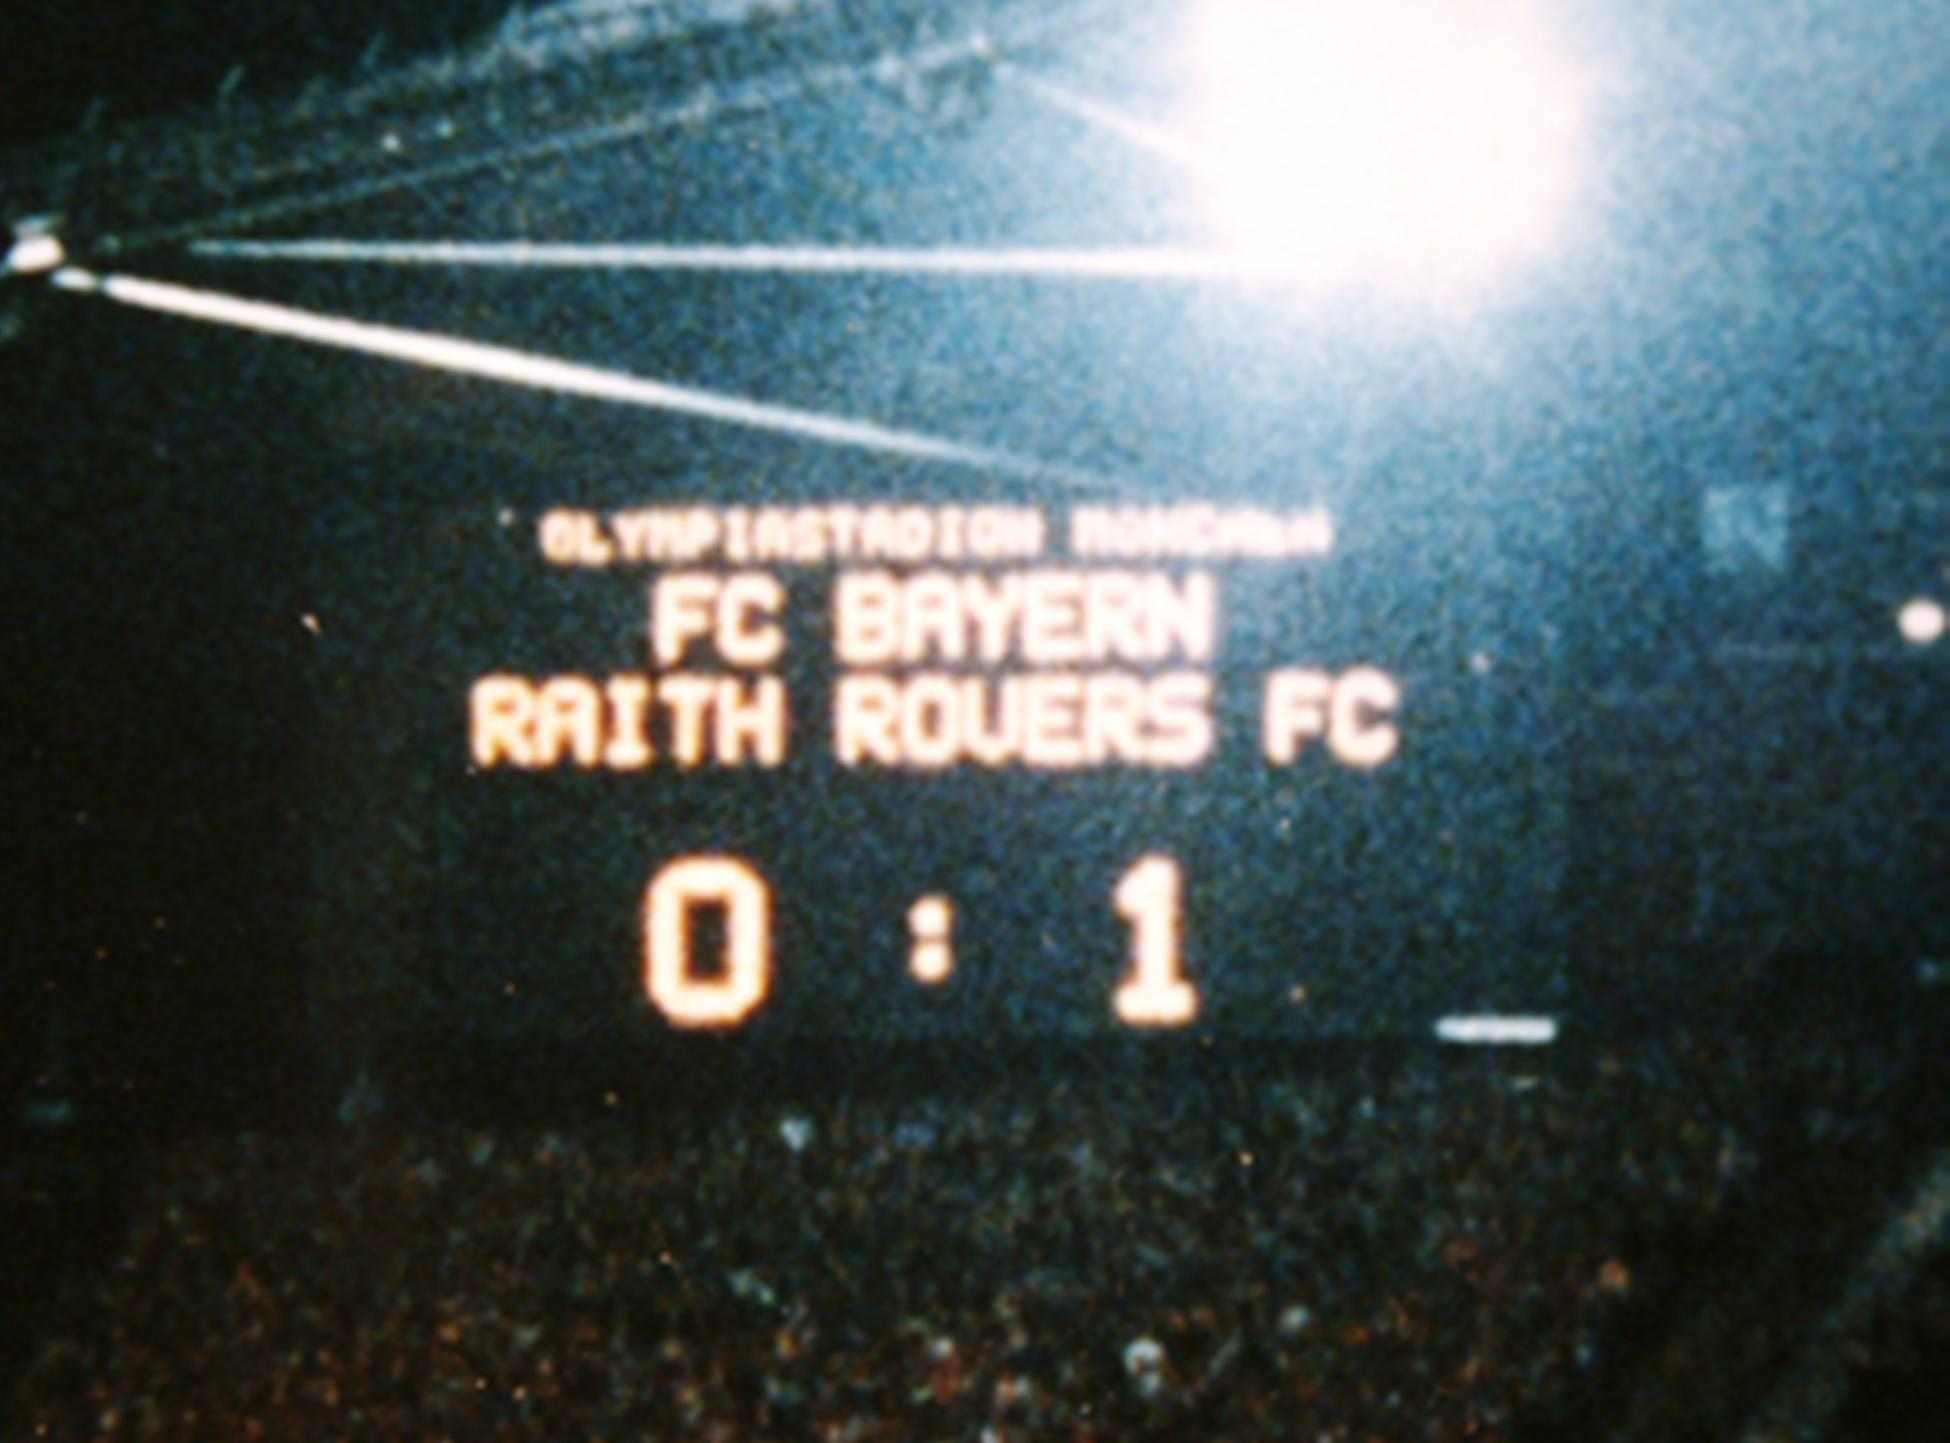
\includegraphics[width=0.65\textwidth,height=0.65\textheight]{images/raith.jpg}

}

\caption{A memorable scoreboard}

\end{figure}
\end{frame}

\begin{frame}{What is Utility}
\protect\hypertarget{what-is-utility-1}{}
\begin{itemize}[<+->]
\tightlist
\item
  The players would prefer a 3-4 result (i.e., 3 for them, 4 for other
  player) to a 2-1 result.
\item
  So this is very much unlike soccer, even though the numbers will often
  feel a lot like soccer scores.
\end{itemize}
\end{frame}

\begin{frame}{What is Utility}
\protect\hypertarget{what-is-utility-2}{}
\begin{itemize}[<+->]
\tightlist
\item
  It's not money, for two distinct reasons.
\item
  First, the players might care how much money the other players get.
\end{itemize}
\end{frame}

\begin{frame}{Utility and Altruism}
\protect\hypertarget{utility-and-altruism}{}
Consider these three situations

\begin{enumerate}
\tightlist
\item
  Billy gets \$90, Suzy gets \$100.
\item
  Billy gets \$100, Suzy gets nothing.
\item
  Billy gets \$110, Suzy gets \$100.
\end{enumerate}

How do you order these in terms of utility to Billy, from highest to
lowest?
\end{frame}

\begin{frame}{Utility and Altruism}
\protect\hypertarget{utility-and-altruism-1}{}
\begin{itemize}[<+->]
\tightlist
\item
  We don't know given just this description.
\item
  If Billy wants Suzy to get money, he might prefer option 1 to option
  2.
\item
  If Billy wants Suzy to not have money, he might prefer option 2 to
  option 3.
\end{itemize}
\end{frame}

\begin{frame}{What is Utility}
\protect\hypertarget{what-is-utility-3}{}
\begin{itemize}[<+->]
\tightlist
\item
  It's not money, for two distinct reasons.
\item
  Second, getting twice as much money typically doesn't produce twice as
  much utility.
\end{itemize}
\end{frame}

\begin{frame}{What is Utility}
\protect\hypertarget{what-is-utility-4}{}
It is, more or less, desirability.

\begin{itemize}[<+->]
\tightlist
\item
  Outcome \(O_1\) has more utility for player \(X\) than outcome \(O_2\)
  iff \(X\) prefers to be in \(O_1\) than \(O_2\).
\end{itemize}
\end{frame}

\begin{frame}{Utility and Numbers}
\protect\hypertarget{utility-and-numbers}{}
\begin{itemize}[<+->]
\tightlist
\item
  Now you might have noticed something odd there.
\item
  We are trying to define this numerical quantity, but we've just told
  you something about when it is bigger or smaller.
\item
  Surely we need to say something more, like how much bigger or smaller
  it is in different situations.
\end{itemize}
\end{frame}

\hypertarget{ordinal-and-cardinal-utility}{%
\section{Ordinal and Cardinal
Utility}\label{ordinal-and-cardinal-utility}}

\begin{frame}{Utility}
\protect\hypertarget{utility-2}{}
A utility function (for a particular agent) is a mapping \(U\) from
situations to numbers satsifying this constraint.

\begin{itemize}[<+->]
\tightlist
\item
  \(U(S_1) > U(S_2)\) iff the agent is better off in \(S_1\) than in
  \(S_2\).
\end{itemize}
\end{frame}

\begin{frame}{Welfare}
\protect\hypertarget{welfare}{}
This isn't part of the formal theory, but we usually implicitly assume
(at least in our narratives), the following principle.

\begin{quote}
The agent is better off in \(S_1\) than in \(S_2\) iff, given a choice
and assuming they are fully informed, they prefer being in \(S_1\) to
\(S_2\).
\end{quote}

That is, we'll usually speak as if a radically subjectivist view of
welfare is correct. I've been doing this already, and I'm going to keep
doing it.
\end{frame}

\begin{frame}{Ordinal Utility}
\protect\hypertarget{ordinal-utility}{}
\begin{itemize}[<+->]
\tightlist
\item
  When we say that we're working with \textbf{ordinal} utility
  functions, really the only principle that applies is the one from two
  slides back.
\item
  Higher utilities are better, i.e., are preferred.
\item
  The term \textbf{ordinal} should make you think of `orders'; all an
  ordinal utility function does is provide a rank \textbf{ordering} of
  the outcomes.
\end{itemize}
\end{frame}

\begin{frame}{Two Functions}
\protect\hypertarget{two-functions}{}
So if we're working in ordinal utility, these two functions describe the
same underlying reality.

\begin{longtable}[]{@{}lcc@{}}
\toprule()
& \(U_1\) & \(U_2\) \\
\midrule()
\endhead
\(O_1\) & 1 & 1 \\
\(O_2\) & 2 & 10 \\
\(O_3\) & 3 & 500 \\
\(O_4\) & 4 & 7329 \\
\bottomrule()
\end{longtable}
\end{frame}

\begin{frame}{Cardinal Utility}
\protect\hypertarget{cardinal-utility}{}
\begin{itemize}[<+->]
\tightlist
\item
  In cardinal utility theory, the differences between the numbers
  matter.
\item
  The numbers now express quantities, and the two functions from the
  previous slide do not represent the same underlying reality.
\end{itemize}
\end{frame}

\begin{frame}{Cardinal Utility (Detail)}
\protect\hypertarget{cardinal-utility-detail}{}
\begin{itemize}[<+->]
\tightlist
\item
  There is a fussy point here that's worth going over.
\item
  Even cardinal utility functions don't come with a scale.
\item
  So two functions with different numbers in them can still express the
  same underlying reality.
\end{itemize}
\end{frame}

\begin{frame}{Cardinal Utility (Detail)}
\protect\hypertarget{cardinal-utility-detail-1}{}
The standard way to put this is that (cardinal) utility is defined only
up to a \textbf{positive, affine transformation}. That means that if
\(U_1\) and \(U_2\) are related by the following formula, then they
represent the same state of affairs.

\[
U_2(o) = aU_1(o) + b \text{ where } a > 0
\]
\end{frame}

\begin{frame}{Celsius and Farenheit}
\protect\hypertarget{celsius-and-farenheit}{}
\begin{itemize}[<+->]
\tightlist
\item
  The main real world cases of scales that are related in this way are
  temperature scales.
\item
  To convert between Celsius and Farenheit you use the formula
  \(F = 1.8C + 32\).
\item
  But the scales are just two ways of representing the same physical
  reality.
\end{itemize}
\end{frame}

\begin{frame}{Cardinal Utility (Detail)}
\protect\hypertarget{cardinal-utility-detail-2}{}
\begin{itemize}[<+->]
\tightlist
\item
  So there is no such thing as one outcome being \emph{twice as good} as
  another.
\item
  But we can say a lot of things about differences.
\end{itemize}
\end{frame}

\begin{frame}{Cardinal Utility (Detail)}
\protect\hypertarget{cardinal-utility-detail-3}{}
\begin{itemize}[<+->]
\tightlist
\item
  If the difference between \(O_1\) and \(O_2\) is the same as the
  difference between \(O_2\) and \(O_3\), that will stay the same under
  any positive affine transformation.
\item
  Indeed, for any \(k\), if the difference between \(O_1\) and \(O_2\)
  is \(k\) times the difference between \(O_2\) and \(O_3\), that will
  stay the same under any positive affine transformation.
\end{itemize}
\end{frame}

\hypertarget{dominance-arguments}{%
\section{Dominance Arguments}\label{dominance-arguments}}

\begin{frame}{A Simple Game}
\protect\hypertarget{a-simple-game}{}
\begin{columns}[T]
\begin{column}{0.4\textwidth}
\begin{table}[!h]
\centering
\begin{tabular}[t]{>{}r|cc}
\toprule
 & Left & Right\\
\midrule
Up & 4, 1 & 2, 0\\
Down & 3, 0 & 1, 1\\
\bottomrule
\end{tabular}
\end{table}
\end{column}

\begin{column}{0.6\textwidth}
Here's how to read this table.

\begin{enumerate}
\tightlist
\item
  Two players, call them Row and Column.
\item
  Row chooses the row, Column chooses the column - between them they
  choose a cell.
\item
  Each cell has two numbers - the first is Row's payout, the second is
  Column's payout.
\end{enumerate}
\end{column}
\end{columns}
\end{frame}

\begin{frame}{Strong Dominance}
\protect\hypertarget{strong-dominance}{}
\begin{columns}[T]
\begin{column}{0.4\textwidth}
\begin{table}[!h]
\centering
\begin{tabular}[t]{>{}r|cc}
\toprule
 & Left & Right\\
\midrule
Up & 4, 1 & 2, 0\\
Down & 3, 0 & 1, 1\\
\bottomrule
\end{tabular}
\end{table}
\end{column}

\begin{column}{0.6\textwidth}
\begin{itemize}[<+->]
\tightlist
\item
  Whatever Column does, Row is better off playing Up rather than Down.
\item
  We say that Up \textbf{strongly dominates} Down.
\end{itemize}
\end{column}
\end{columns}
\end{frame}

\begin{frame}[fragile]{Strong Dominance}
\protect\hypertarget{strong-dominance-1}{}
\begin{columns}[T]
\begin{column}{0.4\textwidth}
\begin{table}[!h]
\centering
\begin{tabular}[t]{>{}r|cc}
\toprule
 & Left & Right\\
\midrule
Up & 4, 1 & 2, 0\\
Middle & 5, 0 & 0, 0\\
Down & 3, 0 & 1, 1\\
\bottomrule
\end{tabular}
\end{table}
\end{column}

\begin{column}{0.6\textwidth}
\begin{itemize}[<+->]
\tightlist
\item
  Adding options doesn't change things.
\item
  Up still dominates Down, even if it isn't always best.
\end{itemize}
\end{column}
\end{columns}
\end{frame}

\begin{frame}[fragile]{Strong Dominance}
\protect\hypertarget{strong-dominance-2}{}
\begin{columns}[T]
\begin{column}{0.4\textwidth}
\begin{table}[!h]
\centering
\begin{tabular}[t]{>{}r|cc}
\toprule
 & Left & Right\\
\midrule
Up & 3, 1 & 0, 0\\
Middle & 2, 0 & 2, 0\\
Down & 0, 0 & 3, 1\\
\bottomrule
\end{tabular}
\end{table}
\end{column}

\begin{column}{0.6\textwidth}
\begin{itemize}[<+->]
\tightlist
\item
  This is \textbf{not} a case of dominance.
\item
  Even though Middle is never the highest value, it isn't dominated by
  any one option.
\end{itemize}
\end{column}
\end{columns}
\end{frame}

\begin{frame}{Strong Dominance}
\protect\hypertarget{strong-dominance-3}{}
Strategy \(S_1\) strongly dominates strategy \(S_2\) if for any strategy
\(S\) by the other player(s), if \(S\) is played, then \(S_1\) returns a
higher payoff than \(S_2\).
\end{frame}

\begin{frame}{Weak Dominance}
\protect\hypertarget{weak-dominance}{}
Strategy \(S_1\) weakly dominates strategy \(S_2\) if for any strategy
\(S\) by the other player(s), if \(S\) is played, then \(S_1\) returns a
payoff that is at least as high \(S_2\), and for some strategy by the
other player(s), \(S_1\) returns a higher payoff than \(S_2\).

\begin{itemize}[<+->]
\tightlist
\item
  The difference is that weak dominance allows for \textbf{ties}.
\end{itemize}
\end{frame}

\begin{frame}{Two Dominance Notions}
\protect\hypertarget{two-dominance-notions}{}
Strong Dominance

\begin{itemize}
\tightlist
\item
  Always better.
\end{itemize}

Weak Dominance

\begin{itemize}
\tightlist
\item
  Never worse.
\item
  Sometimes better.
\end{itemize}
\end{frame}

\begin{frame}[fragile]{Weak Dominance}
\protect\hypertarget{weak-dominance-1}{}
\begin{columns}[T]
\begin{column}{0.4\textwidth}
\begin{table}[!h]
\centering
\begin{tabular}[t]{>{}r|cc}
\toprule
 & Left & Right\\
\midrule
Up & 4, 1 & 2, 0\\
Down & 3, 0 & \textbf{2}, 1\\
\bottomrule
\end{tabular}
\end{table}
\end{column}

\begin{column}{0.6\textwidth}
\begin{itemize}
\tightlist
\item
  I've changed the payoffs in the bottom right cell.
\item
  Now Up does not strongly dominate Down.
\item
  But it does weakly dominate Down.
\end{itemize}
\end{column}
\end{columns}
\end{frame}

\hypertarget{some-famous-games}{%
\section{Some Famous Games}\label{some-famous-games}}

\begin{frame}[fragile]{Prisoners' Dilemma}
\protect\hypertarget{prisoners-dilemma}{}
\begin{table}[!h]
\centering
\begin{tabular}[t]{>{}r|cc}
\toprule
 & Coop & Defect\\
\midrule
Coop & 3, 3 & 0, 5\\
Defect & 5, 0 & 1, 1\\
\bottomrule
\end{tabular}
\end{table}
\end{frame}

\begin{frame}[fragile]{Generic Symmetric Game}
\protect\hypertarget{generic-symmetric-game}{}
\begin{table}[!h]
\centering
\begin{tabular}[t]{>{}r|cc}
\toprule
 & X & Y\\
\midrule
X & a, a & b, c\\
Y & c, b & d, d\\
\bottomrule
\end{tabular}
\end{table}
\end{frame}

\begin{frame}[fragile]{Prisoners' Dilemma}
\protect\hypertarget{prisoners-dilemma-1}{}
\begin{columns}[T]
\begin{column}{0.4\textwidth}
\begin{table}[!h]
\centering
\begin{tabular}[t]{>{}r|cc}
\toprule
 & X & Y\\
\midrule
X & a, a & b, c\\
Y & c, b & d, d\\
\bottomrule
\end{tabular}
\end{table}
\end{column}

\begin{column}{0.6\textwidth}
Ordinal constraints

\begin{itemize}
\tightlist
\item
  \(c > a, d > b\)
\item
  \(a > d\)
\end{itemize}

Cardinal constraints

\begin{itemize}
\tightlist
\item
  \(2a > b + c\)
\end{itemize}
\end{column}
\end{columns}
\end{frame}

\begin{frame}[fragile]{Stag Hunt}
\protect\hypertarget{stag-hunt}{}
\begin{table}[!h]
\centering
\begin{tabular}[t]{>{}r|cc}
\toprule
 & Coop & Defect\\
\midrule
Coop & 5, 5 & 0, 4\\
Defect & 4, 0 & 2, 2\\
\bottomrule
\end{tabular}
\end{table}
\end{frame}

\begin{frame}[fragile]{Stag Hunt}
\protect\hypertarget{stag-hunt-1}{}
\begin{columns}[T]
\begin{column}{0.4\textwidth}
\begin{table}[!h]
\centering
\begin{tabular}[t]{>{}r|cc}
\toprule
 & X & Y\\
\midrule
X & a, a & b, c\\
Y & c, b & d, d\\
\bottomrule
\end{tabular}
\end{table}
\end{column}

\begin{column}{0.6\textwidth}
Ordinal constraints

\begin{itemize}
\tightlist
\item
  \(a > c, d > b\)
\item
  \(a > d\)
\end{itemize}

Cardinal constraints

\begin{itemize}
\tightlist
\item
  \(a + b < c + d\)
\end{itemize}
\end{column}
\end{columns}
\end{frame}

\begin{frame}[fragile]{Battle of the Sexes}
\protect\hypertarget{battle-of-the-sexes}{}
\begin{table}[!h]
\centering
\begin{tabular}[t]{>{}r|cc}
\toprule
 & Row & Col\\
\midrule
Row & 4, 1 & 0, 0\\
Col & 0, 0 & 1, 4\\
\bottomrule
\end{tabular}
\end{table}
\end{frame}

\begin{frame}[fragile]{Battle of the Sexes (relabelled)}
\protect\hypertarget{battle-of-the-sexes-relabelled}{}
\begin{table}[!h]
\centering
\begin{tabular}[t]{>{}r|cc}
\toprule
 & Self & Other\\
\midrule
Self & 0, 0 & 4, 1\\
Other & 1, 4 & 0, 0\\
\bottomrule
\end{tabular}
\end{table}
\end{frame}

\begin{frame}[fragile]{Chicken}
\protect\hypertarget{chicken}{}
\begin{table}[!h]
\centering
\begin{tabular}[t]{>{}r|cc}
\toprule
 & Attack & Retreat\\
\midrule
Attack & -99, -99 & 2, 0\\
Retreat & 0, 2 & 1, 1\\
\bottomrule
\end{tabular}
\end{table}
\end{frame}

\begin{frame}[fragile]{Rock Paper Scissors}
\protect\hypertarget{rock-paper-scissors}{}
\begin{table}[!h]
\centering
\begin{tabular}[t]{>{}r|ccc}
\toprule
 & Rock & Paper & Scissors\\
\midrule
Rock & 0, 0 & -1, 1 & 1, -1\\
Paper & 1, -1 & 0, 0 & -1, 1\\
Scissors & -1, 1 & 1, -1 & 0, 0\\
\bottomrule
\end{tabular}
\end{table}
\end{frame}

\begin{frame}{For Next Time}
\protect\hypertarget{for-next-time}{}
We're jumping ahead to section 2.5 of Bonanno.
\end{frame}



\end{document}
